% Copyright (c) 2015 Daniele Masini - d.masini.it@gmail.com
% Copyright (c) 2016 Daniele Zambelli - daniele.zambelli@gmail.com

\section{Esercizi}

\subsection{Esercizi dei singoli paragrafi}

% \begingroup
% \hypersetup{linkcolor=black}
% \subsubsection*{\ref{sect:rette_parallele} - 
% \nameref{sect:rette_parallele}}
% \endgroup

\subsubsection*{\numnameref{sect:rette_parallele}}

\begin{esercizio}
\label{ese:3.15}
Vero o Falso?
\begin{enumeratea}
\item Due rette parallele tagliate da una trasversale formano \\ 
quattro angoli alterni interni\hfill\boxV\quad\boxF
\item Gli angoli corrispondenti sono a due a due interni o 
esterni\hfill\boxV\quad\boxF
\item Gli angoli interni si trovano da parti opposte rispetto alla 
trasversale\hfill\boxV\quad\boxF
\item Gli angoli esterni si trovano da parti opposte rispetto alla 
trasversale\hfill\boxV\quad\boxF
\item Due rette parallele possono anche 
coincidere\hfill\boxV\quad\boxF
\item La relazione di parallelismo tra rette è una relazione di 
equivalenza\hfill\boxV\quad\boxF
\item Due rette distinte hanno sempre un punto in 
comune\hfill\boxV\quad\boxF
\item Una retta che incontra due rette parallele forma angoli alterni \\
interni supplementari\hfill\boxV\quad\boxF
\item Per ogni retta è possibile tracciare una sola retta 
parallela\hfill\boxV\quad\boxF
\item Se due rette formano con una trasversale due angoli alterni \\
interni allora sono parallele\hfill\boxV\quad\boxF
\item Nel ragionamento per assurdo si nega l'ipotesi per dimostrare che la \\
tesi è vera\hfill\boxV\quad\boxF
\item Ragionando per assurdo si nega la tesi e si ottenere una \\
contraddizione con l'ipotesi\hfill\boxV\quad\boxF
\end{enumeratea}
\hfill [a)~F,\quad b)~F,\quad c)~F,\quad d)~F,\quad e)~V,\quad f)~V,\quad 
g)~F,\quad h)~F,\quad i)~F,\quad j)~F,\quad k)~F,\quad l)~V]
\end{esercizio}

\begin{comment} 

\begin{esercizio}
\label{ese:}
~

\noindent\begin{minipage}{.45\textwidth}

\end{minipage} 
\begin{minipage}{.55\textwidth}
\begin{inaccessibleblock}[Figura: TODO]
\begin{center} \input{\folder } \end{center}
\end{inaccessibleblock}
\end{minipage}
\end{esercizio}

\end{comment}

\begin{esercizio}
\label{ese:3.16}
~

\noindent\begin{minipage}{.45\textwidth}
Nella figura a fianco disegna una parallela e una 
perpendicolare alla retta $r$ passanti per $P$ e una parallela e una 
perpendicolare a $s$ passanti per $Q$.
\end{minipage} 
\begin{minipage}{.55\textwidth}
\begin{inaccessibleblock}[Figura: TODO]
\begin{center} % Copyright (c) 2015 Daniele Masini - d.masini.it@gmail.com

\begin{tikzpicture}[scale=0.9,font=\small, extended line/.style={shorten >=-#1,shorten <=-#1}, extended line/.default=1cm]
\usetikzlibrary{calc, through, intersections}

\begin{scope}
\clip (-0.2,-0.1) rectangle (8.2,2.8);
\coordinate (p) at (3,0.3);
\coordinate (q) at (4.5,0.5);

\draw (0,0) node[above] {$r$} -- (5,3);
\draw (3,3) -- (8,0) node[above] {$s$};

\draw[fill] (p) circle (1.5pt) node[below] {$P$};
\draw[fill] (q) circle (1.5pt) node[below] {$Q$};

\end{scope}

\end{tikzpicture}
 \end{center}
\end{inaccessibleblock}
\end{minipage}
\end{esercizio}

\begin{esercizio}
\label{ese:3.17}
~

\noindent\begin{minipage}{.55\textwidth}
\begin{inaccessibleblock}[Figura: TODO]
\begin{center} % Copyright (c) 2015 Daniele Masini - d.masini.it@gmail.com

\begin{tikzpicture}[scale=0.9,font=\small, extended line/.style={shorten >=-#1,shorten <=-#1}, extended line/.default=1cm]
\usetikzlibrary{calc, through, intersections}

\begin{scope}
\coordinate (p) at (3,0.2);
\coordinate (q) at (4.5,0.5);

\draw (0,0) -- (5,0.5);
\draw (0,1.2) -- (5,1.7);
\draw (1.5,-0.6) -- (3.5,2.4);

\end{scope}

\end{tikzpicture}
 \end{center}
\end{inaccessibleblock}
\end{minipage}
\begin{minipage}{.45\textwidth}
Nella figura in fianco sono state tracciate due rette 
parallele e una trasversale. Segna con un arco gli angoli 
corrispondenti.
\end{minipage} 
\end{esercizio}

\newpage %---------------------------------------------------

\begin{esercizio}
\label{ese:}
~

\noindent\begin{minipage}{.55\textwidth}
\begin{inaccessibleblock}[Figura: TODO]
\begin{center} % Copyright (c) 2015 Daniele Masini - d.masini.it@gmail.com

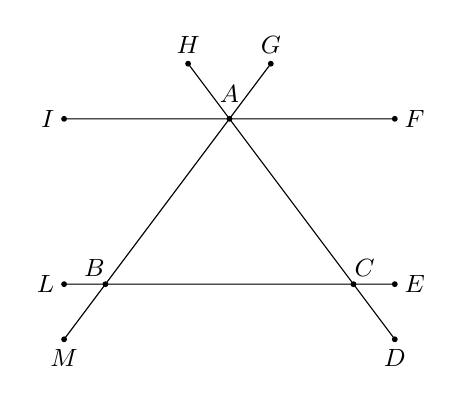
\begin{tikzpicture}[scale=0.7,font=\small, extended line/.style={shorten >=-#1,shorten <=-#1}, extended line/.default=1cm]
\usetikzlibrary{calc, through, intersections}

\begin{scope}
\coordinate (L) at (-3,-3);
\coordinate (E) at (3,-3);
\coordinate (I) at (-3,0);
\coordinate (F) at (3,0);
\coordinate (H) at (-0.75,1);
\coordinate (D) at (3,-4);
\coordinate (G) at (0.75,1);
\coordinate (M) at (-3,-4);

\coordinate (A) at (intersection of H--D and G--M);
\coordinate (B) at (intersection of L--E and G--M);
\coordinate (C) at (intersection of L--E and H--D);

\draw[fill] (I) circle (1.2pt) node[left] {$I$} -- (F) circle (1.2pt) node[right] {$F$};
\draw[fill] (L) circle (1.2pt) node[left] {$L$} -- (E) circle (1.2pt) node[right] {$E$};
\draw[fill] (H) circle (1.2pt) node[above] {$H$} -- (D) circle (1.2pt) node[below] {$D$};
\draw[fill] (G) circle (1.2pt) node[above] {$G$} -- (M) circle (1.2pt) node[below] {$M$};
\draw[fill] (A) circle (1.2pt) node[shift={(0pt,9pt)}] {$A$};
\draw[fill] (B) circle (1.2pt) node[shift={(-4pt,6pt)}] {$B$};
\draw[fill] (C) circle (1.2pt) node[shift={(4pt,6pt)}] {$C$};

\end{scope}

\end{tikzpicture}
 \end{center}
\end{inaccessibleblock}
\end{minipage}
\begin{minipage}{.45\textwidth}
Nella figura a fianco $ABC$ è un triangolo isoscele, $IF$ è 
parallela a $BC$. Individua tutti gli angoli congruenti all'angolo 
$A\widehat{B}C$.
\end{minipage} 
\end{esercizio}

% \begin{esercizio}
% \label{ese:3.19}
% Nella figura~\ref{fig:ese3.19} $ABC$ è un triangolo isoscele, $IF$ è 
% parallela a $BC$. Individua tutti gli angoli congruenti all'angolo 
% $A\widehat{B}C$.
% \end{esercizio}
% 
% \begin{inaccessibleblock}[Figura: TODO]
%  \begin{figure}[htb]
% \centering% Copyright (c) 2015 Daniele Masini - d.masini.it@gmail.com

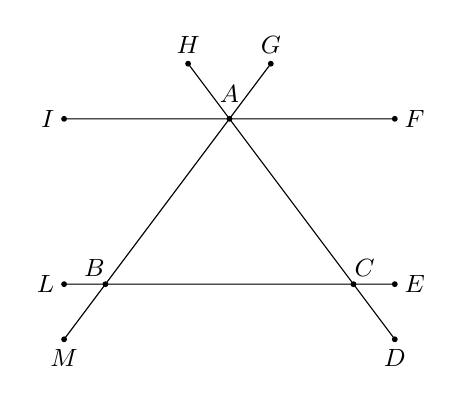
\begin{tikzpicture}[scale=0.7,font=\small, extended line/.style={shorten >=-#1,shorten <=-#1}, extended line/.default=1cm]
\usetikzlibrary{calc, through, intersections}

\begin{scope}
\coordinate (L) at (-3,-3);
\coordinate (E) at (3,-3);
\coordinate (I) at (-3,0);
\coordinate (F) at (3,0);
\coordinate (H) at (-0.75,1);
\coordinate (D) at (3,-4);
\coordinate (G) at (0.75,1);
\coordinate (M) at (-3,-4);

\coordinate (A) at (intersection of H--D and G--M);
\coordinate (B) at (intersection of L--E and G--M);
\coordinate (C) at (intersection of L--E and H--D);

\draw[fill] (I) circle (1.2pt) node[left] {$I$} -- (F) circle (1.2pt) node[right] {$F$};
\draw[fill] (L) circle (1.2pt) node[left] {$L$} -- (E) circle (1.2pt) node[right] {$E$};
\draw[fill] (H) circle (1.2pt) node[above] {$H$} -- (D) circle (1.2pt) node[below] {$D$};
\draw[fill] (G) circle (1.2pt) node[above] {$G$} -- (M) circle (1.2pt) node[below] {$M$};
\draw[fill] (A) circle (1.2pt) node[shift={(0pt,9pt)}] {$A$};
\draw[fill] (B) circle (1.2pt) node[shift={(-4pt,6pt)}] {$B$};
\draw[fill] (C) circle (1.2pt) node[shift={(4pt,6pt)}] {$C$};

\end{scope}

\end{tikzpicture}

% \caption{Esercizio~\ref{ese:3.19}}\label{fig:ese3.19}
% \end{figure}
% \end{inaccessibleblock}

\begin{esercizio}
\label{ese:}
~

\noindent\begin{minipage}{.33\textwidth}
Nella figura a fianco sono state tracciate due rette parallele e una 
trasversale, sapendo che $\alpha=\frac{1}{3}\pi$, dove $\pi$ è 
l'angolo piatto, indica che frazione dell'angolo piatto sono gli 
altri angoli:
\end{minipage} \hfill
\begin{minipage}{.3\textwidth}
$\alpha=\frac{1}{3}\pi$\tab\tab $\beta = \ldots$\\
$\gamma=\ldots$\tab\tab $\delta = \ldots$\\
$\epsilon=\ldots$\tab\tab $\lambda = \ldots$\\
$\phi=\ldots$\tab\tab $\omega = \ldots$
\end{minipage} \hfill
\begin{minipage}{.3\textwidth}
\begin{inaccessibleblock}[Figura: TODO]
\begin{center} % Copyright (c) 2015 Daniele Masini - d.masini.it@gmail.com

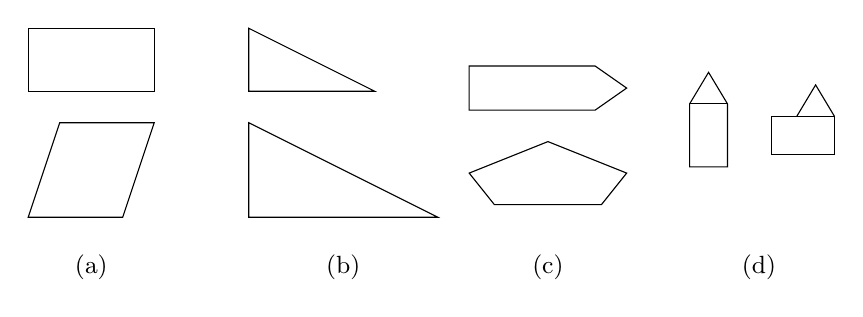
\begin{tikzpicture}[scale=0.8,font=\small]
\usetikzlibrary{calc}

\begin{scope}
\draw (0,0) rectangle (2,1);
\draw (0,-2) -- (1.5,-2) -- (2,-0.5) -- (0.5,-0.5) -- cycle;
\node at (1,-2.8) {(a)};
\end{scope}

\begin{scope}[xshift=3.5cm]
\draw (0,0) -- (0,1) -- (2,0) -- cycle;
\draw (0,-2) -- (0,-0.5) -- (3,-2) -- cycle;
\node at (1.5,-2.8) {(b)};
\end{scope}

\begin{scope}[xshift=7cm]
\begin{scope}[yshift=-0.3cm]
\draw (0,0) -- (0,0.7) -- (2,0.7) -- (2.5,0.35) -- (2,0) -- cycle;
\draw (0,-1) -- (1.25,-0.5) -- (2.5,-1) -- (2.1,-1.5) -- (0.4,-1.5) -- cycle;
\end{scope}
\node at (1.25,-2.8) {(c)};
\end{scope}

\begin{scope}[xshift=10.5cm]
\begin{scope}[yshift=-1.2cm]
\draw (0,0) -- (0,1) -- (0.3,1.5) -- (0.6,1) -- (0.6,0) -- cycle;
\draw (0,1) -- (0.6,1);
\end{scope}
\begin{scope}[xshift=1.3cm, yshift=-1cm]
\draw (0,0) -- (0,0.6) -- (1,0.6) -- (1,0) -- cycle;
\draw (0.4,0.6) -- (0.7,1.1) -- (1,0.6);
\end{scope}
\node at (1.1,-2.8) {(d)};
\end{scope}

\end{tikzpicture}
 \end{center}
\end{inaccessibleblock}
\end{minipage}
\tab\hfill [$\alpha=\dfrac{1}{3}\pi$, $\beta=\dfrac{2}{3}\pi$, 
$\gamma=\dfrac{1}{3}\pi$, $\delta=\dfrac{2}{3}\pi$, 
$\epsilon=\dfrac{1}{3}\pi$, $\lambda=\dfrac{2}{3}\pi$, 
$\phi=\dfrac{1}{3}\pi$, $\omega=\dfrac{2}{3}\pi$]
\end{esercizio}

% \begin{esercizio}
% \label{ese:3.18}
% Nella figura a fianco sono state tracciate due rette parallele e una 
% trasversale, sapendo che $\alpha=\frac{1}{3}\pi$, dove $\pi$ è 
% l'angolo piatto, indica che frazione dell'angolo piatto sono gli 
% altri angoli:\\
% \noindent\begin{minipage}{.5\textwidth}
% $\alpha=\frac{1}{3}\pi$\tab\tab $\beta = \ldots$\\
% $\gamma=\ldots$\tab\tab $\delta = \ldots$\\
% $\epsilon=\ldots$\tab\tab $\lambda = \ldots$\\
% $\phi=\ldots$\tab\tab $\omega = \ldots$
% \end{minipage}\hfil
% \begin{minipage}{.5\textwidth}
% \centering% Copyright (c) 2015 Daniele Masini - d.masini.it@gmail.com

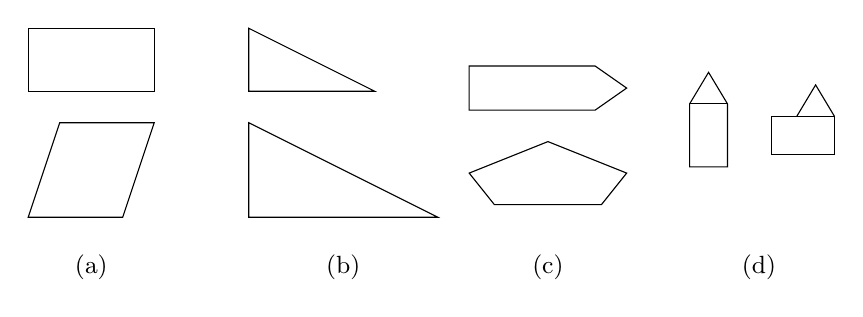
\begin{tikzpicture}[scale=0.8,font=\small]
\usetikzlibrary{calc}

\begin{scope}
\draw (0,0) rectangle (2,1);
\draw (0,-2) -- (1.5,-2) -- (2,-0.5) -- (0.5,-0.5) -- cycle;
\node at (1,-2.8) {(a)};
\end{scope}

\begin{scope}[xshift=3.5cm]
\draw (0,0) -- (0,1) -- (2,0) -- cycle;
\draw (0,-2) -- (0,-0.5) -- (3,-2) -- cycle;
\node at (1.5,-2.8) {(b)};
\end{scope}

\begin{scope}[xshift=7cm]
\begin{scope}[yshift=-0.3cm]
\draw (0,0) -- (0,0.7) -- (2,0.7) -- (2.5,0.35) -- (2,0) -- cycle;
\draw (0,-1) -- (1.25,-0.5) -- (2.5,-1) -- (2.1,-1.5) -- (0.4,-1.5) -- cycle;
\end{scope}
\node at (1.25,-2.8) {(c)};
\end{scope}

\begin{scope}[xshift=10.5cm]
\begin{scope}[yshift=-1.2cm]
\draw (0,0) -- (0,1) -- (0.3,1.5) -- (0.6,1) -- (0.6,0) -- cycle;
\draw (0,1) -- (0.6,1);
\end{scope}
\begin{scope}[xshift=1.3cm, yshift=-1cm]
\draw (0,0) -- (0,0.6) -- (1,0.6) -- (1,0) -- cycle;
\draw (0.4,0.6) -- (0.7,1.1) -- (1,0.6);
\end{scope}
\node at (1.1,-2.8) {(d)};
\end{scope}

\end{tikzpicture}

% \end{minipage}
% \hfill [$\alpha=\dfrac{1}{3}\pi$, $\beta=\dfrac{2}{3}\pi$, 
% $\gamma=\dfrac{1}{3}\pi$, $\delta=\dfrac{2}{3}\pi$, 
% $\epsilon=\dfrac{1}{3}\pi$, $\lambda=\dfrac{2}{3}\pi$, 
% $\phi=\dfrac{1}{3}\pi$, $\omega=\dfrac{2}{3}\pi$]
% \end{esercizio}

\begin{esercizio}
\label{ese:3.20}
Completa ipotesi e tesi e metti in ordine le tre parti della 
dimostrazione:\\
In un triangolo $ABC$, isoscele su base $AB$, si prendano 
rispettivamente su $AC$ e $BC$ i punti $D$ ed $E$ equidistanti da 
$C$. Indicata con $S$ la proiezione di $D$ su $BC$ e con $U$ quella di 
$E$ su $AC$. Dimostrare che il segmento $US$ è parallelo ad $AB$.\\
~\\
\noindent Ipotesi: $AC\cong \ldots$, $D\in AC$, $E\in \ldots$, $S\in 
BC$, $DS\perp BC$, $U\in \ldots$, $EU\perp \ldots$\hfill Tesi: 
$US\parallel AB$.\\
~\\
\noindent\begin{minipage}{.75\textwidth}
\textbf{Parte 1.} I triangoli $CDS$ e $CEU$  hanno: l'angolo 
$\widehat{C}$ in comune, $CD$ \ldots{} $CE$ per \ldots\ldots{}, 
$D\widehat{S}C$ \ldots\ldots\ldots{} perché angoli \ldots\ldots{}, 
quindi tali triangoli sono congruenti per il \ldots\ldots\ldots{}, ne 
segue $CS \ldots CU$ e pertanto $C\widehat{U}S\cong \ldots$\par

\textbf{Parte 2.} Applicando il teorema sulla somma degli angoli 
interni ai triangoli $ABC$ e $CUS$, si ha che $C\widehat{U}S + 
C\widehat{S}U \ldots{} C\widehat{A}B + C\widehat{B}A$ perché 
supplementari dello stesso angolo $\widehat{C}$, ed essendo 
$\widehat{A}$ \dots{} $\widehat{B}$ perché \ldots\ldots\ldots{} ed 
essendo $C\widehat{U}S$ \ldots\ldots{} perché \ldots\ldots\ldots{}, 
risulta che $C\widehat{A}B$ \ldots{} $C\widehat{U}S$ perché 
\ldots\ldots\ldots{}\par

\textbf{Parte 3.} Gli angoli $C\widehat{A}B$ e $C\widehat{U}S$ 
(congruenti perché dimostrato) sono angoli \ldots\ldots rispetto alle 
rette $AB$ e $US$ tagliate dalla trasversale \ldots, quindi le rette 
$AB$ e $US$ sono parallele.
\end{minipage}\hfil
\begin{minipage}{.25\textwidth}
\centering% Copyright (c) 2015 Daniele Masini - d.masini.it@gmail.com

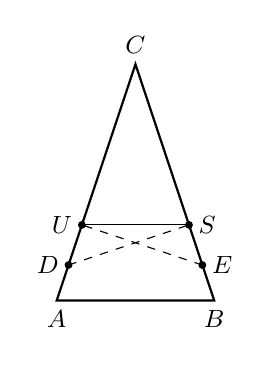
\begin{tikzpicture}[scale=1,font=\small, extended line/.style={shorten >=-#1,shorten <=-#1}, extended line/.default=1cm]
\usetikzlibrary{calc, through, intersections}

\begin{scope}
\coordinate (C) at (0,0);
\coordinate (A) at (-1,-3);
\coordinate (B) at (1,-3);
\coordinate (D) at ($(A)!0.15!(C)$);
\coordinate (E) at ($(B)!0.15!(C)$);
\coordinate (U) at ($(A)!(E)!(C)$);
\coordinate (S) at ($(B)!(D)!(C)$);

\draw[fill] (E) circle (1.2pt) node[right] {$E$};
\draw[fill] (D) circle (1.2pt) node[left] {$D$};
\draw[dashed] (E) -- (U);
\draw[fill] (U) circle (1.2pt) node[left] {$U$};
\draw[dashed] (D) -- (S);
\draw[fill] (S) circle (1.2pt) node[right] {$S$};
\draw (U) -- (S);

\draw[thick] (A) node[below] {$A$} -- (B) node[below] {$B$} -- (C) node[above] {$C$} -- cycle;

\end{scope}

\end{tikzpicture}

\end{minipage}
\end{esercizio}

\begin{esercizio}[Prove invalsi 2005]  %Soluzione: c.
\label{ese:3.21}
$A$, $B$ e $C$ sono tre punti nel piano tali che per i seguenti tre 
angoli, tutti minori di un angolo piatto, valga la relazione 
$B\widehat{A}C=A\widehat{B}C+A\widehat{C}B$. Quanto vale 
$B\widehat{A}C$?
\begin{multicols}{4}
\begin{enumeratea}
\item $70\grado$;
\item $80\grado$;
\item $90\grado$;
\item $100\grado$.
\end{enumeratea}
\end{multicols}
\hfill[c]
\end{esercizio}

\newpage %---------------------------------------------------

\subsubsection*{Dimostra le seguenti affermazioni sul parallelismo 
nei poligoni}

\vspace{-6pt}

\begin{multicols}{2}

\begin{esercizio}
  \label{ese:3.39}
  Due rette parallele tagliate da una trasversale formano otto angoli, 
  uno di essi è $1/3$ dell'angolo retto. Determina le misure degli 
  altri angoli.
\end{esercizio}

\begin{esercizio}
  \label{ese:3.40}
  Siano $\alpha$ e $\beta$ due angoli alterni interni formati da due 
  rette parallele tagliate da una trasversale, dimostra che la 
  bisettrice di $\alpha$ è parallela alla bisettrice di $\beta$.
\end{esercizio}

\begin{esercizio}
  \label{ese:3.41}
  Siano $\alpha$ e $\beta$ due angoli coniugati formati da due rette 
  parallele tagliate da una trasversale, dimostra che la bisettrice di 
  $\alpha$ è perpendicolare alla bisettrice di $\beta$.
\end{esercizio}

\begin{esercizio}
\label{ese:3.24}
Nel triangolo isoscele $ABC$ traccia una parallela alla base $AB$, 
che incontra i lati obliqui in $D$ ed $E$. Dimostra che anche $DCE$ è 
un triangolo isoscele.
\end{esercizio}

\begin{esercizio}
\label{ese:3.26}
Sia $M$ il punto medio del segmento $AB$. Sia $r$ una retta che 
incontra $AB$ in $M$. Sulla retta $r$ da parti opposte rispetto a $M$ 
prendi due punti $C$ e $D$ in modo che $AC\parallel BD$. Dimostra che 
$AC\cong BD$. 
\end{esercizio}

\begin{esercizio}
\label{ese:3.27}
Dal vertice $C$ di un triangolo isoscele $ABC$ conduci la parallela 
alla base $AB$. Dimostra che tale parallela è bisettrice dell'angolo 
esterno in $C$ al triangolo.
\end{esercizio}

\begin{esercizio}
\label{ese:3.28}
Sia $ABC$ un triangolo isoscele di base $AB$. Sia $r$ la semiretta di 
origine $C$ bisettrice dell'angolo formato dal prolungamento di $BC$ 
e dal lato $AC$. Dimostra che la retta $AB$ è parallela a $r$.
\end{esercizio}

\begin{esercizio}
\label{ese:3.29}
Dato il triangolo isoscele $ABC$ di base $AB$ e vertice $C$, prolunga 
la base $AB$ dalla parte di $A$ di un segmento $AD$. Sia $E$ un punto 
interno all'angolo $D\widehat{A}C$ in modo che $E\widehat{A}D\cong 
C\widehat{A}B$. Dimostra che $EA\parallel CB$.
\end{esercizio}

\begin{esercizio}
\label{ese:3.30}
Da ciascun vertice di un triangolo $ABC$ traccia la parallela al lato 
opposto. Detti $D$, $E$ ed $F$ i punti di intersezione delle 
parallele, dimostra che il triangolo $DEF$ ha gli angoli 
ordinatamente congruenti a quelli di $ABC$.
\end{esercizio}

\begin{esercizio}
\label{ese:3.31}
Sia $AD$ la bisettrice dell'angolo in $A$ del triangolo $ABC$. Dal 
punto $D$ traccia la parallela al lato $AB$, essa incontra il lato 
$AC$ in $E$. Dimostra che il triangolo $EDC$ ha gli angoli 
ordinatamente congruenti a quelli di $ABC$. Dimostra anche che $ADE$ 
è un triangolo isoscele.
\end{esercizio}

\begin{esercizio}
\label{ese:3.32}
In un triangolo $ABC$ rettangolo in $A$ traccia l'altezza $AH$ 
relativa all'ipotenusa. Dimostra che il triangolo $ABH$ ha gli angoli 
congruenti a quelli di $ABC$.
\end{esercizio}

\begin{esercizio}
\label{ese:3.35}
In un triangolo $ABC$ sia $E$ il punto di intersezione della 
bisettrice dell'angolo in $B$ con il lato $AC$. Sia $D$ un punto del 
lato $AB$ tale che $DE\cong DB$. Dimostra che $DE\parallel BC$.
\end{esercizio}

\begin{esercizio}
\label{ese:3.37}
Dato il triangolo $ABC$ prolunga il lato $AB$ dalla parte di $A$ di 
un segmento $AD\cong AB$, prolunga poi il lato $AC$ dalla parte di $A$ 
di un segmento $AE\cong AC$. Dimostra che $DE\parallel BC$.
\end{esercizio}

\begin{esercizio}
\label{ese:3.38}
Sia $AM$ la mediana di un triangolo $ABC$. Si prolunghi $AM$ dalla 
parte di $M$ di un segmento $MD$ congruente ad $AM$. Dimostra che 
$CD$ è parallelo ad $AB$.
\end{esercizio}


\begin{esercizio}
\label{ese:3.42}
Disegna due segmenti $AB$ e $CD$ disposti in modo che si incontrino 
nel loro punto medio comune $M$. Congiungi $A$ con $D$ e $B$ con $C$, 
dimostra che $AD$ è parallelo a $CB$.
\end{esercizio}

\begin{esercizio}
\label{ese:3.43}
Disegna un angolo acuto $a\widehat{O}b$ e la sua bisettrice $c$. 
Disegna su $c$ un punto $P$, disegna poi l'asse del segmento $OP$. 
Indica con $Q$ e $R$ i punti di intersezione dell'asse 
rispettivamente con la semiretta $a$ e la semiretta $b$. Dimostra che 
$OQ$ è parallelo a $RP$.
\end{esercizio}

\begin{esercizio}
\label{ese:3.44}
Disegna un angolo convesso $a\widehat{O}b$ e la sua bisettrice $c$. 
Disegna su $c$ un punto $P$, disegna poi le perpendicolari $PR$ e 
$PQ$ rispettivamente alle semirette $a$ e $b$. Dimostra che $c$ è asse 
del segmento $QR$.
\end{esercizio}

\begin{esercizio}
\label{ese:3.45}
Sia $ABC$ un triangolo equilatero. Traccia una parallela al lato $AB$ 
che incontra il lato $BC$ in $D$ e $AC$ in $E$. Dimostra che anche il 
triangolo $CDE$ è equilatero.
\end{esercizio}

\begin{esercizio}
  \label{ese:3.66}
  Dimostra che in un triangolo isoscele la congiungente i punti medi 
  dei lati congruenti è parallela alla base del triangolo.
\end{esercizio}

\end{multicols}

% \begingroup
% \hypersetup{linkcolor=black}
% \subsubsection*{\ref{sect:angoli_interni_triangolo} - 
% \nameref{sect:angoli_interni_triangolo}}
% \endgroup

\subsubsection*{\numnameref{sect:angoli_interni_triangolo}}

\begin{esercizio}
\label{ese:3.47}
Vero o Falso?
\begin{enumeratea}
\item La somma degli angoli interni di un triangolo è congruente a un 
angolo esterno \hfill\boxV\quad\boxF
\item La somma degli angoli interni di un quadrilatero è congruente a 
3 angoli piatti \hfill\boxV\quad\boxF
\item La somma degli angoli esterni di un pentagono è congruente a 5 
angoli piatti\hfill\boxV\quad\boxF
\item La somma degli angoli interni di un triangolo è congruente a 
due angoli retti\hfill\boxV\quad\boxF
\item Un triangolo isoscele non può avere un angolo 
ottuso\hfill\boxV\quad\boxF
\end{enumeratea}
\end{esercizio}

\begin{esercizio}
\label{ese:3.48}
Sia $ABC$ un triangolo equilatero. Si prolunghi $AB$ di un segmento 
$BD$ congruente al lato stesso e si congiunga $D$ con $C$. Si 
dimostri che $ACD$ è un triangolo rettangolo.
\end{esercizio}

\begin{esercizio}
\label{ese:3.49}
Calcola la misura degli angoli di un triangolo $ABC$ sapendo che 
l'angolo interno in $A$ è $4/5$ del relativo angolo esterno e che 
l'angolo interno in $B$ è la metà dell'angolo interno in $A$.
\end{esercizio}

\begin{esercizio}[I Giochi di Archimede 2005]
\label{ese:3.51}
Nella figura seguente, quanto misura l'angolo $\alpha$?  
\end{esercizio}

\begin{inaccessibleblock}[Figura: TODO]
 \begin{figure}[htb]
\centering% Copyright (c) 2015 Daniele Masini - d.masini.it@gmail.com

\begin{tikzpicture}[scale=1.2,font=\small]
\usetikzlibrary{calc}

\begin{scope}
\draw (0,0) node[below left] {$A$} -- (0,2) node[above left] {$C$} -- (1.6,0.6) node[right] {$B$} -- cycle;
\node at (0.6,0.8) {$T_1$};
\end{scope}

\begin{scope}[xshift=3.2cm]
\draw (0,0) node[left] {$A$} -- (0,1.7) node[above left] {$B$} -- (2.3,0) node[right] {$C$} -- cycle;
\node at (0.7,0.6) {$T_2$};
\end{scope}

\begin{scope}[xshift=7cm]
\draw (0,0) node[left] {$A$} -- (1.5,0.7) node[above] {$C$} -- (3,0) node[right] {$B$} -- cycle;
\node at (1.5,0.3) {$T_3$};
\end{scope}

\end{tikzpicture}

\caption{Esercizio~\ref{ese:3.31}}\label{fig:ese3.51}
\end{figure}
\end{inaccessibleblock}

% \begingroup
% \hypersetup{linkcolor=black}
% \subsubsection*{\ref{
% sect:generalizzazione_criteri_congruenza_triangoli} - 
% \nameref{sect:generalizzazione_criteri_congruenza_triangoli}}
% \endgroup

\subsubsection*{\numnameref{sect:generalizzazione_criteri_congruenza_triangoli}}

\begin{esercizio}
\label{ese:3.52}
Vero o Falso?
\begin{enumeratea}
\item Un triangolo rettangolo ha due angoli 
complementari\hfill\boxV\quad\boxF
\item Due triangoli rettangoli sono congruenti se hanno almeno un 
lato congruente\hfill\boxV\quad\boxF
\item Due triangoli rettangoli che hanno un cateto in comune sono 
congruenti\hfill\boxV\quad\boxF
\item Due triangoli rettangoli che hanno l'ipotenusa in comune sono 
congruenti\hfill\boxV\quad\boxF
\item Due triangoli rettangoli isosceli sono sempre 
congruenti\hfill\boxV\quad\boxF
\item Due triangoli rettangoli isosceli che hanno un lato in comune 
sono congruenti\hfill\boxV\quad\boxF
\item Gli angoli acuti di un triangolo rettangolo sono 
complementari\hfill\boxV\quad\boxF
\end{enumeratea}
\end{esercizio}

\newpage %---------------------------------------------------

\subsubsection*{Dimostra le seguenti affermazioni sui teoremi di 
congruenza generalizzati}

\vspace{-6pt}

\begin{multicols}{2}

\begin{esercizio}
\label{ese:3.53}
Dimostra che in triangolo rettangolo gli angoli diversi dall'angolo 
retto sono acuti.
\end{esercizio}

\begin{esercizio}
\label{ese:3.54}
Dimostra che non può esistere un triangolo rettangolo equilatero.
\end{esercizio}

\begin{esercizio}
\label{ese:3.55}
Due triangoli isosceli sono congruenti se hanno congruenti la base e 
l'angolo al vertice.
\end{esercizio}

\begin{esercizio}
\label{ese:3.56}
In un triangolo isoscele, le altezze relative ai lati congruenti sono 
congruenti. 
\end{esercizio}

\begin{esercizio}
\label{ese:3.57}
Due triangoli rettangoli sono congruenti se hanno congruenti un 
cateto e l'altezza relativa all'ipotenusa.
\end{esercizio}

\begin{esercizio}
\label{ese:3.58}
Due triangoli rettangoli sono congruenti se hanno congruenti un 
cateto e la mediana relativa ad esso.
\end{esercizio}

\begin{esercizio}
\label{ese:3.59}
Due triangoli rettangoli sono congruenti se hanno congruenti un 
angolo acuto e la sua bisettrice.
\end{esercizio}

\begin{esercizio}
\label{ese:3.60}
Se due triangoli hanno congruenti due coppie di lati e le mediane 
relative ai lati rimanenti, allora sono congruenti.
\end{esercizio}

\begin{esercizio}
\label{ese:3.69}
Dato un angolo convesso $a\widehat{O}b$ traccia la sua bisettrice 
$c$. Per un punto $P$ della bisettrice traccia la perpendicolare alla 
bisettrice stessa. Chiama $A$ e $B$ i punto di intersezione della 
perpendicolare con i lati $a$ e $b$ dell'angolo convesso. Dimostra 
che $P$ è punto medio di $AB$.
\end{esercizio}

\begin{esercizio}
\label{ese:3.70}
Dato il triangolo isoscele $ABC$, di base $AB$, sul prolungamento 
dell'altezza relativa ad $AB$ prendi un punto $P$. Traccia le rette 
$PA$ e $PB$. Dimostra che l'angolo formato dalle rette $PA$ e $CA$ è 
congruente all'angolo formato dalle rette per $PB$ e $CB$.
\end{esercizio}

% \begin{esercizio}
% \label{ese:3.74}
% Sia $AM$ la mediana di un triangolo $ABC$. Dimostra che se $ABM$ è 
% isoscele il triangolo $ABC$ è rettangolo e viceversa, se il triangolo 
% $ABC$ è rettangolo in $A$ allora $ABM$ è isoscele.
% \end{esercizio}

\begin{esercizio}
\label{ese:3.78}
Nel triangolo $ABC$ traccia la media $CM$ e il suo prolungamento $MD$ 
a piacere. Da $A$ conduci la perpendicolare alla mediana che la 
incontra in $E$, da $B$ conduci un'altra perpendicolare alla mediana 
che la incontra in $F$. Dimostra che i triangoli $AEM$ e $BFM$ sono 
congruenti.
\end{esercizio}

\begin{esercizio}
\label{ese:3.81}
Sia $ABC$ un triangolo acutangolo. Nel semipiano di origine $AB$ che 
non contiene $C$ individua un punto $D$ in modo che 
$B\widehat{A}D\cong C\widehat{B}A$. Dimostra che $CB\parallel AD$. 
Nell'ipotesi in cui $AD\cong CB$ dimostra che anche $AC\parallel BD$.
\end{esercizio}

\end{multicols}

% \begingroup
% \hypersetup{linkcolor=black}
% \subsubsection*{\ref{sect:disuguaglianze_triangoli} - 
% \nameref{sect:disuguaglianze_triangoli}}
% \endgroup

\subsubsection*{\numnameref{sect:disuguaglianze_triangoli}}

\begin{esercizio}
\label{ese:3.82}
Vero o Falso? 
\vspace{-6pt}
\begin{enumeratea}
\item Esiste un triangolo i cui lati misurano 10~cm, 3~cm e 15~cm
\hfill\boxV\quad\boxF
\item Un triangolo isoscele può essere ottusangolo
\hfill\boxV\quad\boxF
\item Dati tre segmenti di cui almeno uno maggiore degli altri è 
sempre possibile \\
costruire un triangolo che ha lati congruenti ai tre segmenti dati
\hfill\boxV\quad\boxF
\item Dai tre segmenti di cui due uguali e uno maggiore è sempre possibile \\
costruire un triangolo isoscele che ha lati congruenti ai tre segmenti dati
\hfill\boxV\quad\boxF
\item In un triangolo rettangolo l'ipotenusa è minore della somma dei 
due cateti
\hfill\boxV\quad\boxF
\item Un triangolo di perimetro 100~cm non può avere un lato di 60~cm
\hfill\boxV\quad\boxF
\item In un triangolo l'angolo che si oppone al lato maggiore è 
sempre acuto\hfill\boxV\quad\boxF
\item In un triangolo rettangolo i cateti sono sempre congruenti
\hfill\boxV\quad\boxF
\item In un triangolo rettangolo l'ipotenusa può essere congruente ad 
un cateto
\hfill\boxV\quad\boxF
\item Un triangolo può avere due lati disuguali e due angoli uguali
\hfill\boxV\quad\boxF
\end{enumeratea}
\hfill [a)~F,\quad b)~V,\quad c)~F,\quad d)~F,\quad e)~V,\quad f)~V,\quad 
g)~F,\quad h)~F,\quad i)~F,\quad j)~V]
\end{esercizio}

\subsubsection*{Dimostra le seguenti affermazioni}

\begin{multicols}{2}

\begin{esercizio}
\label{ese:3.84}
Dimostra che in ogni triangolo rettangolo l'ipotenusa è maggiore di 
ciascun cateto.
\end{esercizio}

\begin{esercizio}
\label{ese:3.86}
In un triangolo ottusangolo il lato opposto all'angolo ottuso è 
maggiore di ciascuno degli altri due lati.
\end{esercizio}

\begin{esercizio}
\label{ese:3.87}
Dimostra che in un triangolo il doppio di un lato è minore del 
perimetro del triangolo. 
\end{esercizio}

\begin{esercizio}
\label{ese:3.92}
In un triangolo ogni lato è minore del semiperimetro.
\end{esercizio}

\begin{esercizio}
\label{ese:3.93}
In un triangolo l'altezza è minore della semisomma dei due lati che 
hanno un vertice in comune con essa.
\end{esercizio}

\begin{esercizio}
\label{ese:3.98}
Esternamente al triangolo $ABC$ prendi un punto $D$. Congiungi $D$ 
con $A$, con $B$ e con $C$. Dimostra che il perimetro di $ABC$ è 
minore del doppio della somma delle distanze di $D$ dai tre vertici 
del triangolo.
\end{esercizio}

\begin{esercizio}
\label{ese:3.99}
Nel triangolo $ABC$ traccia la mediana $AM$ relativa al lato $BC$, 
dimostra che $AM$ è minore della semisomma degli altri due lati $AB$ 
e $AC$. (Prolunga la mediana di un segmento congruente alla mediana 
stessa.)
\end{esercizio}

\begin{esercizio}
\label{ese:3.102}
Dato un triangolo $ABC$ in cui $AB<AC$ traccia l'altezza $AH$ 
relativa alla base $BC$. Dimostra che l'angolo $H\widehat{A}C$ è 
maggiore dell'angolo $H\widehat{A}B$.
\end{esercizio}

\begin{esercizio}
\label{ese:3.106}
Due triangoli rettangoli hanno un cateto in comune e l'angolo opposto 
al cateto in comune è maggiore nel primo triangolo. Dimostra che 
l'ipotenusa del primo triangolo è minore di quella del secondo.
\end{esercizio}

\begin{esercizio}
\label{ese:3.109}
Disegna un punto $D$ interno a un triangolo $ABC$ qualsiasi. Dimostra 
che $B\widehat{D}C>B\widehat{A}C$.
\end{esercizio}

\end{multicols}

\begin{esercizio}[Prove invalsi 2004]
\label{ese:3.112}
~\\
\noindent\begin{minipage}{0.6\textwidth}
Le rette $r$ ed $s$ sono tagliate dalla trasversale $t$. Quale delle 
seguenti condizioni permette di stabilire, per qualunque posizione di 
$t$, che $r$ ed $s$ sono parallele?\\
Gli angoli \ldots{}
\begin{enumeratea}
\item 1 e 5 sono supplementari;
\item 2 e 8 sono uguali;
\item 3 e 7 sono supplementari;
\item 4 e 7 sono uguali.
\end{enumeratea}
\end{minipage}\hfil
\begin{minipage}{0.4\textwidth}
\centering% Copyright (c) 2015 Daniele Masini - d.masini.it@gmail.com

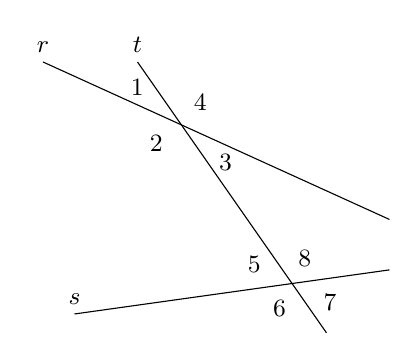
\begin{tikzpicture}[scale=0.8,font=\small, extended line/.style={shorten >=-#1,shorten <=-#1}, extended line/.default=1cm]
\usetikzlibrary{calc, through, intersections}

\begin{scope}
\coordinate (s1) at (0,0);
\coordinate (s2) at (5,0.7);
\coordinate (r1) at (-0.5,4);
\coordinate (r2) at (5,1.5);
\coordinate (t1) at (4,-0.3);
\coordinate (t2) at (1,4);

\coordinate (p1) at (intersection of s1--s2 and t1--t2);
\coordinate (p2) at (intersection of r1--r2 and t1--t2);

\node[black] at ([shift={(-0.7,0.6)}]p2) {$1$};
\node[black] at ([shift={(0.3,0.35)}]p2) {$4$};
\node[black] at ([shift={(-0.4,-0.3)}]p2) {$2$};
\node[black] at ([shift={(0.7,-0.6)}]p2) {$3$};

\node[black] at ([shift={(-0.6,0.3)}]p1) {$5$};
\node[black] at ([shift={(0.2,0.4)}]p1) {$8$};
\node[black] at ([shift={(-0.2,-0.4)}]p1) {$6$};
\node[black] at ([shift={(0.6,-0.3)}]p1) {$7$};

\draw (r1) node[above] {$r$} -- (r2);
\draw (s1) node[above] {$s$} -- (s2);
\draw (t1) -- (t2) node[above] {$t$};

\end{scope}

\end{tikzpicture}

\end{minipage}
\hfill [b]
\end{esercizio}

\begin{esercizio}[Prove invalsi 2006]
\label{ese:3.113}
Per un triangolo ottusangolo qualsiasi, quale delle seguenti 
affermazioni è vera?
\begin{enumeratea}
\item La somma dei suoi due angoli più piccoli è minore dell'angolo 
più grande.
\item Il punto di incontro degli assi dei lati è certamente interno 
al triangolo.
\item Il triangolo è necessariamente isoscele.
\item Il triangolo può essere rettangolo.
\end{enumeratea}
\hfill [a]
\end{esercizio}

\begin{esercizio}[Prove invalsi 2006]
\label{ese:3.114}
~\\
\noindent\begin{minipage}{0.65\textwidth}
$r$ ed $s$ sono due rette parallele tagliate da una trasversale $t$. 
Quale tra le seguenti proposizioni è vera qualunque sia la posizione 
di $t$?
Gli angoli $\alpha$ e $\beta$ sono \ldots{}
\begin{enumeratea}
\item supplementari;
\item uguali;
\item complementari;
\item corrispondenti.
\end{enumeratea}
\end{minipage}\hfil
\begin{minipage}{0.35\textwidth}
\centering% Copyright (c) 2015 Daniele Masini - d.masini.it@gmail.com

\begin{tikzpicture}[scale=1,font=\small]
\usetikzlibrary{calc}

\begin{scope}
\draw[fill] (0,0) coordinate (c) circle (1pt) node[above right] {$C$};
\draw[fill] (1.7,0) coordinate (d) circle (1pt) node[above right] {$D$};
\draw[thick, blue, ->] (c) -- (d);
\draw[fill] (-0.4,-0.8) coordinate (a) circle (1pt) node[above right] {$A$};
\draw[fill] (0.7,-1.7) coordinate (b) circle (1pt) node[above right] {$B$};
\end{scope}

\end{tikzpicture}

\end{minipage}
\hfill [a]
\end{esercizio}

\begin{esercizio}[Prove invalsi 2004]
\label{ese:3.115}
In un triangolo, le misure dei lati sono $a$, $b$ e $c$, con $a = b < 
c$. Detti $\alpha$, $\beta$ e $\gamma$ gli angoli interni del 
triangolo, rispettivamente opposti ai lati $a$, $b$ e $c$, quale 
delle seguenti affermazioni è vera?
\begin{multicols}{4}
\begin{enumeratea}
\item $\alpha = \gamma$;
\item $\beta = \gamma$;
\item $\gamma > \alpha$;
\item $\alpha > \beta$.
\end{enumeratea}
\end{multicols}
\hfill [c]
\end{esercizio}

\begin{esercizio}[Prove invalsi 2010]
\label{ese:3.116}
Un triangolo ha un lato di 6~cm e uno di 10~cm. Quale tra le seguenti 
non può essere la misura della lunghezza del terzo lato?
\begin{multicols}{4}
\begin{enumeratea}
\item $\np{6,5}$~cm;
\item 10~cm;
\item $\np{15,5}$~cm;
\item 17~cm.
\end{enumeratea}
\end{multicols}
\hfill [d]
\end{esercizio}

\begin{esercizio}[Prove invalsi 2005]
\label{ese:3.117}
In un triangolo isoscele l'angolo al vertice è metà dell'angolo alla 
base. Quanto misurano gli angoli del triangolo?
\begin{multicols}{4}
\begin{enumeratea}
\item $72\grado$, $72\grado$, $36\grado$;
\item $30\grado$, $60\grado$, $90\grado$;
\item $36\grado$, $36\grado$, $72\grado$;
\item $90\grado$, $45\grado$, $45\grado$.
\end{enumeratea}
\end{multicols}
\hfill [a]
\end{esercizio}
